%!TEX TS-program = xelatex
\documentclass[]{friggeri-jj-cv}
\usepackage{wrapfig}
\addbibresource{bibliography.bib}
\begin{document}
\header{JJ}{Merelo}
       {Professor at the University of Granada}

% In the aside, each new line forces a line break
\begin{aside}
  \section{about}
    Depto. Arquitectura y Tecnología de Computadores
    C/ Daniel Saucedo Aranda s/n
    18071 Granada
    Spain
    ~
    \href{mailto:jjmerelo@gmail.com}{jjmerelo@gmail.com}
    \href{http://twitter.com/jjmerelo}{{\tt @jjmerelo}}
    \href{https://stackoverflow.com/users/891440/jjmerelo}{StackOverflow}
    \href{http://scholar.google.com/citations?user=gFxqc64AAAAJ}{Google Scholar}
    \href{https://www.researchgate.net/profile/JJ_Merelo}{ResearchGate}
    \href{https://figshare.com/authors/Juan_J_Merelo/541327}{FigShare}
   \href{https://github.com/JJ}{GitHub}
   \href{http://lnkd.in/dBVqYPa}{LinkedIn}
   \href{http://rpubs.com/jjmerelo/}{RPubs}
   \href{http://gitxiv.com/users/jj-merelo}{GitXiv}
   \href{https://www.npmjs.com/~jjmerelo}{NPM}
   \href{http://search.cpan.org/~jmerelo/}{CPAN}
   \href{https://modules.raku.org/search/?q=author%3A%22JMERELO%22}{Raku ecosystem}
   \href{https://profile.codersrank.io/user/jj}{Codersrank profile}
  \section{languages}
    Bilingual Spanish/English
    Spoken French \& Italian
    German, Dutch notions
  \section{programming}
  {\color{red} \large $\varheartsuit$} Agile mindset
  {\color{red} \large $\varheartsuit$} Raku \& Perl
  {\color{red} $\varheartsuit$} Python \& JavaScript/{\tt node.js}
    Lua, Ruby, shell, CSS3 \& HTML5, R, Scala, Ansible, Go.
  \end{aside}

\section{interests}

Evolutionary algorithms, complex networks, social networks, emerging
computing, literary engineering, distributed computing, stealth
computing, computational intelligence in games, machine learning,
repository mining, CI/CD/automation engineering, agile programming,
higher education.

\section{education}

\begin{entrylist}
  \entry
    {1994}
    {Ph.D. {\normalfont in Physics} magna cum laude}
    {University of Granada}
    {\emph{Evolutionary neural networks}}
  \entry
    {1988}
    {M.Sc. {\normalfont in Physics} magna cum laude}
    {University of Granada}
    {Majoring in Physics, Specialization in Theoretical Physics}
  \entry
    {1983–1988}
    {Avg B+}
    {University of Granada}
    {B. Sc. in Physics}
\end{entrylist}

\section{experience}

My main job has always been as a researcher and (since 2009 tenured)
professor at the univesity of Granada. I have also held part-time
positions in a company, Civista, for a short period of time, as well
as consulting gigs with different, mainly local, companies. In the
last two years I've volunteered to help with
\href{https://raku.org}{Raku programming language}, mainly creating
adn managing the documentation.

\begin{entrylist}
  \entry
    {1988-2009}
    {Assistant professor}
    {University of Granada}
    {\emph{Dept. of Computer Architecture}}
  \entry
    {2009-}
    {Full professor.}
    {University of Granada}
    {\emph{Dept. of Computer Architecture}}
    \entry
    {2008-2017}
    {Director.}
    {University of Granada}
    {\href{http://osl.ugr.es}{\emph{Free Software Office}}}
    \entry
    {2017}
    {Member}
    {Microsoft Technical Advisory Group, Cloud CLI \& SDK Tools}
    {1-year position, for consultations on the state and evolution of
      cloud tools}
    \entry
    {April-May '18}
    {Grantee}
    {The Perl Foundation}
    {2-month grant to work on the Perl 6 documentation}
    \entry
    {2018-}
    {Documenter-in-chief}
    {Raku}
    {Documentation in Raku is a separate effort from
      development. Being in charge of the documentation obviously
      writing the documentation, but also working with other
      volunteers to improve it as well as in the tooling to test and
      deploy the documentation}

        \entry
    {2020-}
    {Steering Council}
    {Raku}
    {Elected as part of the 7 member Steering Council, which is the
      last resort for solving problems and disputes in the Raku
      community, and acts as {\em product owner} of the language}
\end{entrylist}

\begin{wrapfigure}{L}{0.20\linewidth}
    \centering
    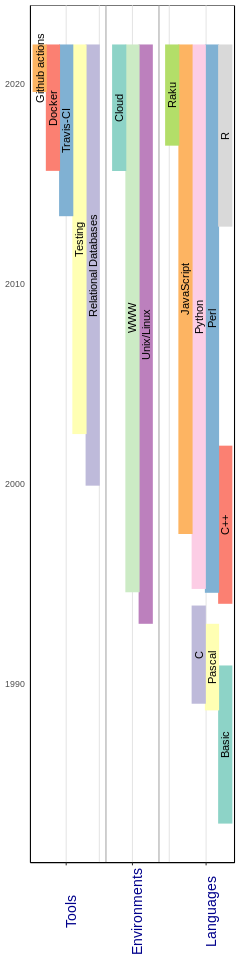
\includegraphics[width=0.19\textwidth]{img/timeline.png}
    \caption{Programming and tools timeline}
\end{wrapfigure}

\newpage

\section{books}

These and other books are included in my
\href{https://amazon.com/author/jjmerelo}{Amazon's author page},
including books in Spanish, edited proceedings and coauthored books.

\begin{entrylist}
  \entry
    {2013}
    {Manuel the Magnificent Mechanical Man}
    {\href{http://www.amazon.com/dp/B00ED084BK/}{Kindle Direct Publishing}}
    {\href{http://jj.github.io/hoborg}{An open source novel} and a
      Perl module}

  \entry
    {2016}
    {Granada On}
    {\href{https://www.amazon.com/Granada-Beaten-Track-explorations-Andalusia/dp/1523257083}{Kindle Direct Publishing}}
    {\href{http://github.com/JJ/granada-off}{An open source travel book}}

  \entry
    {2017}
    {Learning to program with Perl6}
    {\href{https://www.amazon.com/Learning-program-Perl-Getting-programming/dp/1521795789/ref=sr_1_1?ie=UTF8&qid=1518685809&sr=8-1}{Kindle Direct Publishing}}
    {\href{http://github.com/JJ/perl6em}{A book to learn Perl6 (now
        Raku) from scratch}}

    \entry
    {October 2019}
    {Perl 6 Quick Syntax Reference}
    {\href{https://www.apress.com/gp/book/9781484249550}{APress}}
    {As part of the ``Quick Sybtax'' series, a pocket guide to learn
      the language and start working with it. }

  \entry
    {October 2020}
    {Raku recipes}
    {\href{https://www.apress.com/gp/book/9781484262573}{APress}}
    {As part of the ``Recipes'' series, a more advanced book that
      solves real-world problem with Raku. }

  \end{entrylist}

\section{awards}
\begin{entrylist}
 \entry
    {2009}
    {Bubok literary prize}
    {\href{http://cultura.elpais.com/cultura/2009/05/06/actualidad/1241560804_850215.html}{1st
        edition of this prize}}
    {Awarded to the novel {\tt lujoyglamour.net}.}
 \entry
    {April 2014}
    {CS4HS award}
    {\href{http://cs4hs.com}{Computer Science 4 High Schools}}
    {developed as the \href{http://cs4hs.ugr.es}{Google/UGR Tech Campus for Girls}}
 \entry
    {April 2017}
    {CS4HS award}
    {\href{http://cs4hs.com}{Computer Science 4 High Schools}}
    {Development starting on June 1st, 2017, with a program for
      creating a community of practice for K12 and high school
      teachers}
    \entry
    {February 2019}
    {\href{https://summerofcode.withgoogle.com/organizations/4713351599357952/}{Google
        Summer of Code funding}}
    {{\href{https://www.perlfoundation.org/}{The Perl Foundation}}
    {Participation in the selection of ideas, mentors and students
      participating in GSoC, as well as mentoring some projects}

\end{entrylist}

\newpage

\section{libraries and other released software}

\begin{entrylist}
  \entry
    {2004-}
    {{\tt Algorithm::Evolutionary}}
    {\href{http://search.cpan.org/dist/Algorithm-Evolutionary/}{http://search.cpan.org/dist/Algorithm-Evolutionary/}}
    {Evolutionary Algorithm library in
      perl. Check \href{http://search.cpan.org/~jmerelo/}{All my modules at CPAN}}

    \entry
    {2014-}
    {{\tt NodEO}}
    {\href{https://npmjs.org/package/nodeo}{https://www.npmjs.org/package/nodeo}}
    {Evolutionary Algorithm Library in JavaScript for NodeJS}

    \entry
    {2020-}
    {{\tt Test::Script}}
    {\href{https://github.com/JJ/raku-test-script}{github.com/JJ/raku-test-script}}
    {A module to test the output of Raku scripts, which can be used to include in CI
    workflows non-modular applications.}

\end{entrylist}

\section{international projects}

\begin{entrylist}
  \entry
    {2001-2005}
    {{\sf DREAM} Distributed Resource Evolutionary Algorithm Machine}
    {\href{http://www.soc.napier.ac.uk/~benp/dream/dream.htm}{Dream
        Project page}}
    {Peer to peer, asynchronous, evolutionary computation}
  \entry
    {2012-15}
    {Muses project}
    {\href{https://musesproject.eu/}{Muses Project Page}}
    {Mobile, user centered, adaptive security}
    \entry
    {2018-2022}
    {EduBots}
    {\href{https://edubots.eu}{Edubots}}
    {Computational intelligence and learning analytics in higher education}
\end{entrylist}

\section{publications}

I published my first paper before graduation:

\cite{merelo88}

and my first paper in a journal a few years later, getting already
into parallel computing:

\cite{parallel90}
I was working for a few years applying Kohonen's Self-Organizing Map to protein structure prediction

\cite{jjproteng}
and it hit pay dirt, since 20 years after it gathers more than a
thousand references (and growing). Let's not dwell in the past
and talk about current developments. I was PhD advisor for JLJ Laredo,
who continued with DREAM development. This paper is a good example of
our work in the area.

\cite{evag:gpem}
but his work raised several issues about how asynchronous distributed
evolutionary computing worked, which we addressed in this paper in
which I am the first author.

\cite{jj:2008:PPSN}
problems similar to what we found in our work on browser-based
evolutionary algorithms.

\cite{agajaj}
long before browser-based botnets were discovered. I also started to
work with the Mastermind Puzzle in 1996.

\cite{jj-ppsn96}
setting the state of the art several times until today. Our latest hints at
literary engineering.

\cite{2014arXiv1403.3084G}

Lately, I'm getting interested in mining GitHub repositories looking
at the health of communities and their evolution and other
issues. This is the first paper I published on the topic:

\cite{2016arXiv160107862M}

but, since that one, we have produced new results on the complex
nature of repositories using the same repository-mining techniques.

One of my last papers focuses on creating an architecture for
deploying evolutionary algorithms, an optimization technique, to the
cloud.

\cite{GARCIAVALDEZ2021234}

These regular contributions to journals and open publications have
netted close to 7000 citations and and $H=37$ according to Google Scholar.

%\printbibliography

\end{document}
